\chapter{引言}
\label{cha:intro}

\section{研究意义}
\label{sec:first}
视觉是人类感知世界的最直接和重要的方法,光线通过眼睛、视网膜、大脑等器官的处理,最终
形成我们所感知的一幅幅图像。通过这些图像,光怪陆离的大自然直接呈现在我们面前。计算机视觉
的主要研究目标是在计算机上实现达到甚至超过人类视觉系统的功能。当前,计算机视觉领域是
计算机科学的重要和热门研究领域。根据经验,我们在观察图像时,一般会将注意力集中在图像中的某些
感兴趣区域,例如,人、动物、汽车、文字等。一般将这类对象成为前景对象或显著性对象,相反,图像中的另外一部分则
称为背景。背景减除,或前景检测,是指在图像中取出背景部分,或提取图像中的前景对象的一种技术。
例如,在图~\ref{fig:1}中,~\ref{fig:subfig1}中为输入图像,~\ref{fig:subfig2}中为背景减除技术提取的前景对象,其中用白色表示前景区域,黑色表示背景区域。\par
\begin{figure}[h]
  \centering%
  \subcaptionbox{输入图像\label{fig:subfig1}}[3cm] %标题的长度,超过则会换行,如下一个小图。
    {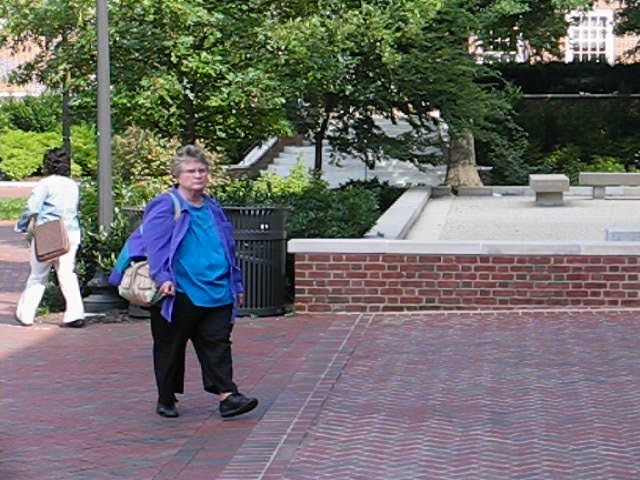
\includegraphics[height=3cm]{p2.jpg}}%
  \hspace{4em}%
  \subcaptionbox{背景减除结果,白色为前景,黑色为背景\label{fig:subfig2}}
      {
\includegraphics[height=3cm]{gtp2.png}}
  \caption{背景减除示例}
  \label{fig:1}
\end{figure}
作为计算机尝试分析并理解图像的第一步,背景减除是视频监控、目标识别与跟踪、手势识别等应用领域中重要的预处理步骤。
人类的视觉系统与生俱来具有这种能力,然而在计算机上实现视频图像中的背景减除却十分困难。主要的
困难在于:
 \begin{itemize}
    \item 噪声干扰。在环境噪声的干扰下,我们得到的图像中可能包含一些噪声,这些噪声会对前景提取的准确度造成重要的影响。例如
    在雨雪天气或者夜间拍摄的图像中,存在亮度不足,雨雪对前景判别产生干扰等问题;
    \item 前景的多样性和不确定性。在不同的场景下,前景对象的定义存在不确定性,例如,在一张汽车广告画中汽车是前景对象,然而同样是汽车,
    在车模的特写照片中却成为背景。
    \item 动态背景,在视频背景减除中,我们在判别前景和背景时一般假设背景区域的像素是静止,而运动的像素
    则属于前景。然而,在实际应用中,这一假设并不总是成立。例如视频中被风吹动摇摆的树叶,喷泉,以及流动的水面等。这些对象虽然是运动
    的,但实际却属于背景;
    \item 相机的运动,在早期的视频背景减除技术研究中,一般假设相机是静止的。然而,随着移动计算平台,例如手机、手持摄像机、智能机器人等,
    的出现,移动相机拍摄视频中的背景减除技术研究越来越重要。在移动相机拍摄的视频中,区分相机运动和前景运动是一项困难的工作。
  \end{itemize}

\par
综上所述,背景减除技术是计算机视觉研究中一个非常热门的课题。提高背景减除技术的准确度和速度对于众多
应用具有十分重要的意义。
\section{相关工作概述}
\label{sec:second}

\subsection{静止相机情况下的视频背景减除}
\label{sec:staticCamera}
在早期的视频背景减除技术研究中,一般假设摄像机是静止的。基于这一假设,通过分析相邻图像帧中像素的变化,可以有效的识别运动的前景。最直接的方法是通过对视频中前后两帧图像进行差分运算,得到

\subsection{移动相机情况下的视频背景减除}
\label{sec:movingCamera}

\subsection{图像显著性分析}
\label{sec:imageSaliency}


\subsection{图像填充技术}
\label{sec:imageInpainting}

\section{论文研究内容}
\label{sec:contents}


\section{本文的组织结构}
\label{sec:hierarchy} 